\documentclass{standalone}

\usepackage[spanish]{babel} %------- Entorno de latex en español -------%
\usepackage[utf8]{inputenc} %------- Acentos nativos -------%
%------- Importar gráficas de ruta específica -------%
\usepackage{graphicx} %------- Para especificar tamaño de gráficos -------%
\graphicspath{{../img/}}
%----------------------------------------------------%
%---------- Formas para diagramas de flujo ----------%
\usepackage{tikz}
\usetikzlibrary{shapes, arrows, positioning}
\tikzset{font={\fontsize{11pt}{12}\selectfont}}
\tikzstyle{redondeado} = [rectangle, rounded corners, text width=2cm, minimum height=2em, minimum width=4em, text centered, draw=black, fill=red!30]
\tikzstyle{cuadro} = [rectangle, text width=2cm, minimum height=2em, minimum width=4em, text centered, draw=black, fill=cyan!20]
\tikzstyle{inclinado} = [trapezium, trapezium left angle=70, trapezium right angle=110, text width=1.5cm, minimum height=2em, minimum width=4em, text badly centered, draw=black, fill=green!30]
\tikzstyle{decision} = [diamond, text width=1.5cm, minimum height=2em, minimum width=4em, text badly centered, draw=black, fill=yellow!30]
\tikzstyle{burbuja} = [ellipse, text width=2cm, minimum height=2em, minimum width=4em, text badly centered, draw=black, fill=brown!30]
\tikzstyle{circulo} = [circle, text width=1mm, minimum height=1mm, minimum width=1mm, draw=black, fill=blue!30]
\tikzstyle{linea} = [draw, line width=0.2em, -latex']
%----------------------------------------------------%

\begin{document}

  \begin{tikzpicture}[auto, node distance = 1cm]
    \node [redondeado] (A) {Inicio};
    \node [circulo, right = of A] (X1) {};
    \node [cuadro, right = of X1] (B) {Activar registro de huella};
    \node[above=0.5em of B] (Y1) {
\includegraphics[width=3em]{ingenieria_proyecto/activador_grabador.eps}};
    \node [inclinado, right = of B] (C) {Colocar huella};
    \node[above=0.5em of C] (Y2) {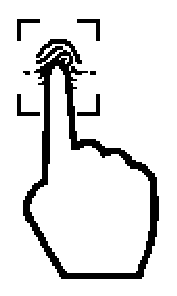
\includegraphics[width=2em]{ingenieria_proyecto/mano_biometrico.eps}};
    \node [cuadro, right = of C] (D) {Verificar huella};
    \node[above=0.5em of D] (Y3) {
\includegraphics[width=2em]{ingenieria_proyecto/reconociendo_huella.eps}};
    \node [decision, below = of D] (E) {Huella válida};
    \node [cuadro, below = of E] (F) {Raspberry envía huella};
    \node[left=0.5em of F] (Y4) {
\includegraphics[width=2em]{ingenieria_proyecto/raspberry.eps}};
    \node [cuadro, below = of F] (G) {Servidor recibe huella};
    \node[below=0.5em of G] (Y5) {
\includegraphics[width=2em]{ingenieria_proyecto/servidor.eps}};
    \node [cuadro, left = of G] (H) {Huella se almacena en la base de datos};
    \node[below=0.5em of H] (Y6) {
\includegraphics[width=2em]{ingenieria_proyecto/huella.eps}};
    \node [cuadro, left = of H, text width = 4cm] (I) {Base de datos notifica cambios al sistema de control de accesos};
    \node[below=0.5em of I] (Y7) {
\includegraphics[width=2em]{ingenieria_proyecto/base_datos.eps}};
    \node [redondeado, left = of I] (J) {Fin};

    \path [linea] (A) -> (X1);
    \path [linea] (X1) -> (B);
    \path [linea] (B) -> (C);
    \path [linea] (C) -> (D);
    \path [linea] (D) -> (E);
    \path [linea] (E) -| node {No} (X1);
    \path [linea] (E) -> node {Si} (F);
    \path [linea] (F) -> (G);
    \path [linea] (G) -> (H);
    \path [linea] (H) -> (I);
    \path [linea] (I) -> (J);
  \end{tikzpicture}

\end{document}